\documentclass[12pt,a4paper]{article}
\usepackage[utf8]{vietnam}
\usepackage{amsmath,amssymb}
\usepackage{tabularx}
\usepackage{tikz}
\usetikzlibrary{calc,angles,quotes,arrows.meta}
\usepackage{xcolor}
\usepackage{enumitem}
\usepackage{fancyhdr}
\usepackage[top=1.0cm, bottom=1.1cm, left=1.3cm, right=1.3cm]{geometry}
\usepackage[dethi]{ex_test}
\SAOPTN{widthSA=3.2,heightSA=0.62}

\setlength{\headheight}{15pt}
\setlength{\parskip}{1.5pt}

\pagestyle{fancy}
\fancyhf{}
\lhead{\textit{Trường THCS Sơn Tây -- Hướng dẫn giải Đề KSCL Lớp 9 Lần 1}}
\rhead{\textit{Năm học 2026 -- 2027 | Môn Toán (Mã đề: 01)}}
\cfoot{\thepage/4}

\begin{document}

% =============================================================================
% TRANG 1: TIÊU ĐỀ & PHẦN I TRẮC NGHIỆM
% =============================================================================
\begin{center}
  {\bfseries\large TRƯỜNG THCS SƠN TÂY \hfill ĐỀ KHẢO SÁT CHẤT LƯỢNG LỚP 9 -- LẦN 1}\\
  \vspace{1mm}
  {\bfseries\Large HƯỚNG DẪN GIẢI CHI TIẾT VÀ BAREM THANG ĐIỂM}\\
  \vspace{1mm}
  \textit{Năm học 2026 -- 2027 | Môn: TOÁN (MÃ ĐỀ: 01) | Thời gian làm bài: 90 phút}
\end{center}
\vspace{-1.5mm}
\hrule
\vspace{2.5mm}

\noindent\textbf{\large I. PHẦN TRẮC NGHIỆM (2,0 điểm)}

\textit{Mỗi câu trả lời đúng được 0,25 điểm.}

\begin{center}
\begin{tabular}{|c|c|c|c|c|c|c|c|c|}
\hline
\textbf{Câu} & \textbf{1} & \textbf{2} & \textbf{3} & \textbf{4} & \textbf{5} & \textbf{6} & \textbf{7} & \textbf{8} \\
\hline
\textbf{Đáp án} & \textbf{D} & \textbf{C} & \textbf{B} & \textbf{D} & \textbf{C} & \textbf{D} & \textbf{B} & \textbf{A} \\
\hline
\end{tabular}
\end{center}
\vspace{1.5mm}

\noindent\textbf{Giải thích chi tiết phương án chọn:}
\begin{itemize}[leftmargin=18pt, itemsep=3.5pt, parsep=0pt]
  \item \textbf{Câu 1 (Chọn D):} Phương trình bậc nhất hai ẩn có dạng $ax + by = c$, trong đó các hệ số $a, b$ không đồng thời bằng 0. Ở phương án D, cả hai hệ số của $x$ và $y$ đều bằng 0 ($0x - 0y = -1$) nên không phải phương trình bậc nhất hai ẩn.
  \item \textbf{Câu 2 (Chọn C):} Thay cặp số $(x; y) = (4; 2)$ vào hệ phương trình ở phương án C:
  $\begin{cases} 4 + 2 = 6 \\ 4 - 2 = 2 \end{cases}$ (thỏa mãn cả hai phương trình).
  \item \textbf{Câu 3 (Chọn B):} Tọa độ giao điểm $M$ của $d_1$ và $d_2$ là nghiệm của hệ phương trình:
  \[
    \begin{cases}
      5x + y = 7 \\
      -x - 3y = 21
    \end{cases}
    \iff
    \begin{cases}
      y = 7 - 5x \\
      -x - 3(7 - 5x) = 21
    \end{cases}
    \iff
    \begin{cases}
      14x = 42 \\
      y = 7 - 5x
    \end{cases}
    \iff
    \begin{cases}
      x = 3 \\
      y = -8
    \end{cases}
    \implies M(3; -8).
  \]
  \item \textbf{Câu 4 (Chọn D):} $(2x - 4)(3x + 6) = 0 \iff \left[\begin{aligned} 2x - 4 &= 0 \\ 3x + 6 &= 0 \end{aligned}\right. \iff \left[\begin{aligned} x &= 2 \\ x &= -2 \end{aligned}\right.$.\\
  Tổng các nghiệm của phương trình là: $2 + (-2) = 0$.
  \item \textbf{Câu 5 (Chọn C):} Biển số R.306 là biển báo tốc độ tối thiểu cho phép, có hiệu lực bắt buộc các phương tiện vận hành với tốc độ không nhỏ hơn trị số ghi trên biển ($60\,\text{km/h}$). Do đó $a \ge 60$.
  \item \textbf{Câu 6 (Chọn D):} Trong $\Delta ABC$ vuông tại $A$, cạnh huyền $BC = \sqrt{AB^2 + AC^2} = \sqrt{3^2 + 4^2} = 5$.\\
  Theo định nghĩa tỉ số lượng giác của góc nhọn $C$: $\cos C = \dfrac{AC}{BC} = \dfrac{4}{5}$.
  \item \textbf{Câu 7 (Chọn B):} Trong tam giác $MNP$ vuông tại $M$:\\
  $\cos N = \dfrac{MN}{NP} = \dfrac{5}{10} = \dfrac{1}{2} \implies \widehat{N} = 60^\circ$.\\
  Vì tam giác vuông tại $M$ nên $\widehat{P} = 90^\circ - \widehat{N} = 90^\circ - 60^\circ = 30^\circ$.\\
  Suy ra: $\widehat{N} - \widehat{P} = 60^\circ - 30^\circ = 30^\circ$.
  \item \textbf{Câu 8 (Chọn A):} Vì hai góc phụ nhau nên: $\cos 65^\circ = \sin 25^\circ$ và $\sin 85^\circ = \cos 5^\circ$.\\
  Thay vào biểu thức ta được:
  \[
    \sin 25^\circ + \cos 5^\circ - \cos 65^\circ - \sin 85^\circ = \sin 25^\circ + \cos 5^\circ - \sin 25^\circ - \cos 5^\circ = 0.
  \]
\end{itemize}

\newpage

% =============================================================================
% TRANG 2: CÂU 9 & CÂU 10
% =============================================================================
\noindent\textbf{\large II. PHẦN TỰ LUẬN (8,0 điểm)}

\vspace{1.5mm}
\noindent\textbf{Câu 9 (2,0 điểm).} Giải các phương trình sau:

\begin{enumerate}[label=\arabic*), leftmargin=18pt, itemsep=3pt, parsep=0pt]
  \item $(x - 4)^2 = 5x - 20$ \hfill \textbf{(1,0 điểm)}
  \begin{itemize}[leftmargin=16pt, itemsep=1.5pt, parsep=0pt]
    \item Chuyển vế và đặt nhân tử chung:\\
    $(x - 4)^2 = 5(x - 4) \iff (x - 4)^2 - 5(x - 4) = 0$ \dotfill \textbf{0,25 điểm}
    \item Biến đổi phương trình tích:\\
    $(x - 4)(x - 4 - 5) = 0 \iff (x - 4)(x - 9) = 0$ \dotfill \textbf{0,25 điểm}
    \item Giải từng trường hợp:\\
    $\left[\begin{aligned} x - 4 &= 0 \\ x - 9 &= 0 \end{aligned}\right. \iff \left[\begin{aligned} x &= 4 \\ x &= 9 \end{aligned}\right.$ \dotfill \textbf{0,25 điểm}
    \item Kết luận: Vậy tập nghiệm của phương trình là $S = \{4; 9\}$. \dotfill \textbf{0,25 điểm}
  \end{itemize}

  \item $\dfrac{1}{2x - 1} - \dfrac{3}{2x + 1} = \dfrac{6x - 3}{4x^2 - 1}$ \hfill \textbf{(1,0 điểm)}
  \begin{itemize}[leftmargin=16pt, itemsep=1.5pt, parsep=0pt]
    \item Điều kiện xác định: $4x^2 - 1 \neq 0 \iff (2x - 1)(2x + 1) \neq 0 \iff x \neq \pm \dfrac{1}{2}$. \dotfill \textbf{0,25 điểm}
    \item Quy đồng mẫu thức chung $4x^2 - 1 = (2x - 1)(2x + 1)$ và khử mẫu:\\
    $(2x + 1) - 3(2x - 1) = 6x - 3$ \dotfill \textbf{0,25 điểm}
    \item Khai triển và thu gọn:\\
    $2x + 1 - 6x + 3 = 6x - 3 \iff -4x + 4 = 6x - 3 \iff -10x = -7 \iff x = \dfrac{7}{10}$. \dotfill \textbf{0,25 điểm}
    \item Đối chiếu ĐKXĐ: $x = \dfrac{7}{10}$ thỏa mãn điều kiện xác định.\\
    Vậy nghiệm của phương trình là $x = \dfrac{7}{10}$. \dotfill \textbf{0,25 điểm}
  \end{itemize}
\end{enumerate}

\vspace{2.5mm}
\hrule
\vspace{2.5mm}

\noindent\textbf{Câu 10 (1,0 điểm).}
\begin{enumerate}[label=\arabic*), leftmargin=18pt, itemsep=3pt, parsep=0pt]
  \item Giải bất phương trình: $\dfrac{x - 3}{5} < \dfrac{2x + 17}{3}$ \hfill \textbf{(0,5 điểm)}
  \begin{itemize}[leftmargin=16pt, itemsep=1.5pt, parsep=0pt]
    \item Nhân cả hai vế với $15 > 0$ để khử mẫu: $3(x - 3) < 5(2x + 17)$ \dotfill \textbf{0,25 điểm}
    \item Khai triển và chuyển vế:\\
    $3x - 9 < 10x + 85 \iff 3x - 10x < 85 + 9 \iff -7x < 94 \iff x > -\dfrac{94}{7}$.\\
    Vậy tập nghiệm của bất phương trình là $x > -\dfrac{94}{7}$. \dotfill \textbf{0,25 điểm}
  \end{itemize}

  \item Cho $a < b$. Chứng minh rằng: $-3a + 2024 > -3b + 2023$ \hfill \textbf{(0,5 điểm)}
  \begin{itemize}[leftmargin=16pt, itemsep=1.5pt, parsep=0pt]
    \item Vì $a < b$ và $-3 < 0$, nhân cả hai vế với $-3$ bất đẳng thức đổi chiều: $-3a > -3b$. \dotfill \textbf{0,25 điểm}
    \item Cộng 2023 vào hai vế: $-3a + 2023 > -3b + 2023$.\\
    Mặt khác, vì $2024 > 2023$ nên $-3a + 2024 > -3a + 2023$.\\
    Theo tính chất bắc cầu, suy ra: $-3a + 2024 > -3b + 2023$ (đpcm). \dotfill \textbf{0,25 điểm}
  \end{itemize}
\end{enumerate}

\newpage

% =============================================================================
% TRANG 3: CÂU 11 & CÂU 12
% =============================================================================
\noindent\textbf{Câu 11 (2,0 điểm).} \textit{Giải bài toán bằng cách lập hệ phương trình:}

Hai ngăn của một kệ sách có tổng cộng 450 cuốn sách. Nếu chuyển 30 cuốn từ ngăn thứ nhất sang ngăn thứ hai thì số sách ở ngăn thứ nhất gấp 2 lần số sách ở ngăn thứ hai. Tính số sách ở mỗi ngăn lúc đầu?

\vspace{1.5mm}
\noindent\textbf{Lời giải chi tiết:}
\begin{itemize}[leftmargin=16pt, itemsep=2.5pt, parsep=0pt]
  \item Gọi số sách ở ngăn thứ nhất lúc đầu là $x$ (cuốn, điều kiện: $x \in \mathbb{N}^*, x > 30$).\\
  Gọi số sách ở ngăn thứ hai lúc đầu là $y$ (cuốn, điều kiện: $y \in \mathbb{N}^*$). \dotfill \textbf{0,25 điểm}
  \item Vì tổng số sách ở cả hai ngăn là 450 cuốn nên ta có phương trình:
  \[
    x + y = 450 \quad (1)
  \] \dotfill \textbf{0,50 điểm}
  \item Khi chuyển 30 cuốn từ ngăn thứ nhất sang ngăn thứ hai:
  \begin{itemize}[leftmargin=14pt, itemsep=1pt]
    \item Số sách ở ngăn thứ nhất còn lại: $x - 30$ (cuốn).
    \item Số sách ở ngăn thứ hai lúc này: $y + 30$ (cuốn).
  \end{itemize}
  Vì khi đó số sách ở ngăn thứ nhất gấp 2 lần số sách ở ngăn thứ hai nên ta có phương trình:
  \[
    x - 30 = 2(y + 30) \iff x - 30 = 2y + 60 \iff x - 2y = 90 \quad (2)
  \] \dotfill \textbf{0,50 điểm}
  \item Từ (1) và (2) ta có hệ phương trình:
  \[
    \begin{cases}
      x + y = 450 \\
      x - 2y = 90
    \end{cases}
    \iff
    \begin{cases}
      3y = 360 \\
      x = 450 - y
    \end{cases}
    \iff
    \begin{cases}
      x = 330 \\
      y = 120
    \end{cases}
    \text{ (thỏa mãn điều kiện)}.
  \] \dotfill \textbf{0,50 điểm}
  \item Kết luận: Vậy lúc đầu ngăn thứ nhất có 330 cuốn sách, ngăn thứ hai có 120 cuốn sách. \dotfill \textbf{0,25 điểm}
\end{itemize}

\vspace{2.5mm}
\hrule
\vspace{2.5mm}

\noindent\textbf{Câu 12 (2,0 điểm).} 
\par\noindent
\begin{minipage}[t]{0.62\linewidth}
Một người đứng ở vị trí điểm $C$ trên mặt đất cách chân tháp ăng-ten một khoảng $CD = 120\,\text{m}$. Biết rằng người ấy nhìn thấy đỉnh tháp với góc $\widehat{AOB} = 32^\circ$ so với đường nằm ngang, khoảng cách từ mắt người đó đến mặt đất là $OC = 1{,}6\,\text{m}$.

Tính chiều cao $AD$ của tháp ăng-ten (kết quả làm tròn đến hai chữ số ở phần thập phân).
\end{minipage}\hfill
\begin{minipage}[t]{0.36\linewidth}
\vspace{-2mm}
\begin{center}
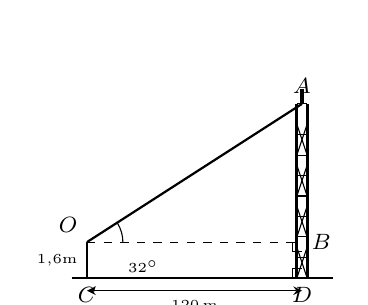
\begin{tikzpicture}[scale=0.65, >=stealth]
  \draw[thick] (-0.3,0) -- (4.8,0);
  \node[below] at (0,0) {\footnotesize $C$};
  \node[below] at (4.2,0) {\footnotesize $D$};
  
  \draw[thick] (0,0) -- (0,0.7);
  \node[above left] at (0,0.7) {\footnotesize $O$};
  \node[left] at (0,0.35) {\tiny $1{,}6\text{m}$};
  
  \coordinate (O) at (0,0.7);
  \coordinate (B) at (4.2,0.7);
  \coordinate (D) at (4.2,0);
  \coordinate (A) at (4.2,3.4);
  
  \draw[dashed] (O) -- (B);
  \node[right] at (B) {\footnotesize $B$};
  \draw[thick] (O) -- (A) node[above]{\footnotesize $A$};
  
  % Tháp AD
  \draw[line width=1.1pt] (4.1,0) -- (4.1,3.4);
  \draw[line width=1.1pt] (4.3,0) -- (4.3,3.4);
  \draw[line width=1.2pt] (4.2,3.4) -- (4.2,3.7);
  \foreach \y in {0, 0.4, 0.8, 1.2, 1.6, 2.0, 2.4, 2.8, 3.4} {
    \draw (4.1,\y) -- (4.3,\y);
  }
  \foreach \y in {0, 0.8, 1.6, 2.4} {
    \draw (4.1,\y) -- (4.3,\y+0.6);
    \draw (4.3,\y) -- (4.1,\y+0.6);
  }
  
  \draw (B) ++(0,-0.18) -- ++(-0.18,0) -- ++(0,0.18);
  \draw (D) ++(0,0.18) -- ++(-0.18,0) -- ++(0,-0.18);
  
  \draw (O) ++(0.7,0) arc (0:31.6:0.7);
  \node at (1.1,0.22) {\tiny $32^\circ$};
  
  \draw[<->] (0,-0.25) -- (4.2,-0.25);
  \node[below] at (2.1,-0.25) {\tiny $120\,\text{m}$};
\end{tikzpicture}
\end{center}
\end{minipage}

\vspace{1mm}
\noindent\textbf{Lời giải chi tiết:}
\begin{itemize}[leftmargin=16pt, itemsep=2.5pt, parsep=0pt]
  \item Tứ giác $OCDB$ có $\widehat{C} = \widehat{D} = \widehat{B} = 90^\circ$ nên là hình chữ nhật.\\
  Suy ra: $OB = CD = 120\,\text{m}$ và $BD = OC = 1{,}6\,\text{m}$. \dotfill \textbf{0,50 điểm}
  \item Xét tam giác $AOB$ vuông tại $B$, theo định nghĩa tỉ số lượng giác của góc nhọn $\widehat{AOB} = 32^\circ$:
  \[
    \tan \widehat{AOB} = \frac{AB}{OB} \implies AB = OB \cdot \tan 32^\circ = 120 \cdot \tan 32^\circ \approx 74{,}9843\,\text{m}.
  \] \dotfill \textbf{0,75 điểm}
  \item Chiều cao của tháp ăng-ten là đoạn $AD$:
  \[
    AD = AB + BD \approx 74{,}9843 + 1{,}6 = 76{,}5843\,\text{m} \approx 76{,}58\,\text{m}.
  \]
  Vậy chiều cao của tháp ăng-ten khoảng $76{,}58\,\text{m}$. \dotfill \textbf{0,75 điểm}
\end{itemize}

\newpage

% =============================================================================
% TRANG 4: CÂU 13 & BẢNG MA TRẬN ĐIỂM
% =============================================================================
\noindent\textbf{Câu 13 (1,0 điểm).}
\begin{enumerate}[label=\arabic*), leftmargin=18pt, itemsep=2.5pt, parsep=0pt]
  \item Giải phương trình: $\dfrac{4x}{4x^2 - 8x + 7} + \dfrac{3x}{4x^2 - 10x + 7} = 1$ \hfill \textbf{(0,5 điểm)}
  \begin{itemize}[leftmargin=16pt, itemsep=1.5pt, parsep=0pt]
    \item Nhận xét $x = 0$ không là nghiệm. Với $x \neq 0$, chia cả tử và mẫu của mỗi phân thức cho $x$:
    \[
      \frac{4}{4x - 8 + \dfrac{7}{x}} + \frac{3}{4x - 10 + \dfrac{7}{x}} = 1.
    \]
    Đặt $t = 4x + \dfrac{7}{x} - 9$. Phương trình trở thành: $\dfrac{4}{t + 1} + \dfrac{3}{t - 1} = 1$ ($t \neq \pm 1$). \dotfill \textbf{0,25 điểm}
    \item Quy đồng mẫu và khử mẫu:
    \[
      4(t - 1) + 3(t + 1) = (t + 1)(t - 1) \iff 7t - 1 = t^2 - 1 \iff t^2 - 7t = 0 \iff \left[\begin{aligned} t &= 0 \\ t &= 7 \end{aligned}\right. \text{ (TMĐK)}.
    \]
    \begin{itemize}[leftmargin=12pt, itemsep=1pt]
      \item Với $t = 0$: $4x + \dfrac{7}{x} - 9 = 0 \iff 4x^2 - 9x + 7 = 0$ có $\Delta = -31 < 0 \implies$ phương trình vô nghiệm.
      \item Với $t = 7$: $4x + \dfrac{7}{x} - 9 = 7 \iff 4x^2 - 16x + 7 = 0 \iff x_1 = \dfrac{7}{2}; \ x_2 = \dfrac{1}{2}$ (thỏa mãn mẫu $\neq 0$).
    \end{itemize}
    Vậy tập nghiệm của phương trình là $S = \left\{\dfrac{1}{2}; \dfrac{7}{2}\right\}$. \dotfill \textbf{0,25 điểm}
  \end{itemize}

  \item Cho các số $a, b, c$ dương. Chứng minh rằng:
  $\dfrac{a}{bc} + \dfrac{b}{ca} + \dfrac{c}{ab} \ge \dfrac{1}{a} + \dfrac{1}{b} + \dfrac{1}{c}$ \hfill \textbf{(0,5 điểm)}
  \begin{itemize}[leftmargin=16pt, itemsep=1.5pt, parsep=0pt]
    \item Vì $a, b, c > 0$, áp dụng bất đẳng thức Cauchy cho hai số dương:
    \[
      \frac{a}{bc} + \frac{b}{ca} \ge 2\sqrt{\frac{a}{bc} \cdot \frac{b}{ca}} = 2\sqrt{\frac{1}{c^2}} = \frac{2}{c} \quad (1)
    \] \dotfill \textbf{0,25 điểm}
    \item Tương tự ta có: $\dfrac{b}{ca} + \dfrac{c}{ab} \ge \dfrac{2}{a} \quad (2)$ và $\dfrac{c}{ab} + \dfrac{a}{bc} \ge \dfrac{2}{b} \quad (3)$.\\
    Cộng vế theo vế ba bất đẳng thức (1), (2), (3) ta được:
    \[
      2\left(\frac{a}{bc} + \frac{b}{ca} + \frac{c}{ab}\right) \ge 2\left(\frac{1}{a} + \frac{1}{b} + \frac{1}{c}\right)
      \implies \frac{a}{bc} + \frac{b}{ca} + \frac{c}{ab} \ge \frac{1}{a} + \frac{1}{b} + \frac{1}{c} \quad (\text{đpcm}).
    \]
    Dấu đẳng thức xảy ra khi và chỉ khi: $\dfrac{a}{bc} = \dfrac{b}{ca} = \dfrac{c}{ab} \iff a = b = c > 0$. \dotfill \textbf{0,25 điểm}
  \end{itemize}
\end{enumerate}

\vspace{2mm}
\hrule
\vspace{2mm}

% --- BẢNG TỔNG HỢP CƠ CẤU ĐIỂM ---
\noindent\textbf{\large BẢNG TỔNG HỢP CƠ CẤU ĐIỂM TOÀN BÀI THI:}
\begin{center}
\small
\renewcommand{\arraystretch}{1.1}
\begin{tabular}{|l|p{11.8cm}|c|}
\hline
\textbf{Phần thi} & \textbf{Nội dung kiến thức đánh giá} & \textbf{Điểm} \\
\hline
\textbf{Phần I} & 8 câu hỏi trắc nghiệm khách quan 4 lựa chọn (0,25đ/câu) & \textbf{2,0 đ} \\
\hline
\textbf{Câu 9} & Phương trình tích (1,0đ) và phương trình chứa ẩn ở mẫu (1,0đ) & \textbf{2,0 đ} \\
\hline
\textbf{Câu 10} & Bất phương trình bậc nhất (0,5đ) và so sánh, BĐT cơ bản (0,5đ) & \textbf{1,0 đ} \\
\hline
\textbf{Câu 11} & Toán thực tế giải bài toán bằng cách lập hệ phương trình (kệ sách) & \textbf{2,0 đ} \\
\hline
\textbf{Câu 12} & Toán thực tế góc nâng tháp ăng-ten (tỉ số lượng giác góc nhọn) & \textbf{2,0 đ} \\
\hline
\textbf{Câu 13} & Phương trình ẩn ở mẫu quy về bậc 2 (0,5đ) và BĐT Cauchy 3 biến (0,5đ) & \textbf{1,0 đ} \\
\hline
\multicolumn{2}{|r|}{\textbf{TỔNG CỘNG TOÀN BÀI THI:}} & \textbf{10,0 đ} \\
\hline
\end{tabular}
\end{center}

\vspace{1mm}
\begin{center}
  \textbf{--- HẾT ---}
\end{center}

\end{document}

